\chapter{Einleitung}
Die \gls{HDR}-Bildgebung ist eines von vielen interessanten Problemen in dem aufstrebenden Forschungsgebiet \textit{Computational Photography}. Ziel dieser Arbeit ist die Fusion mehrerer Bilder mit verschiedener Belichtungszeit -- zu einem einzigen Bild mit deutlich vergrößertem Dynamikumfang.
 
\section{Motivation}


Während viele Arbeiten sich nur mit der pixelweisen Fusion der Bilddaten auseinander setzen, schlagen Debevec und Malik \cite{paper} vor, gleichzeitig auch noch die Antwortkurve des Bildaufnahmeprozesses, d.h. der verwendeten Kamera mitzuschätzen (siehe \autoref{fig:antwortkurve}). Dies bietet den klaren Vorteil, die Bildfusion auch ohne vorherige radiometrische Kalibration des Aufnahmeequipments durchführen zu können. Als mathematisches Werkzeug zur Formulierung des Verfahrens dient hierbei ein gemeinsames Energiefunktional, dass einen Ähnlichkeits- und einen  Glattheitsterm besitzt. Während der Ähnlichkeitsterm unter Berücksichtigung der mitgeschätzten Antwortkurve die Beziehung zwischen den Einzelaufnahmen und dem gesuchten HDR-Bild herstellt, sorgt der Glattheitsterm für eine hinreichend glatte Antwortkurve, die auch aus radiometrischer Sicht Sinn macht.


\begin{figure}
  \begin{center}
    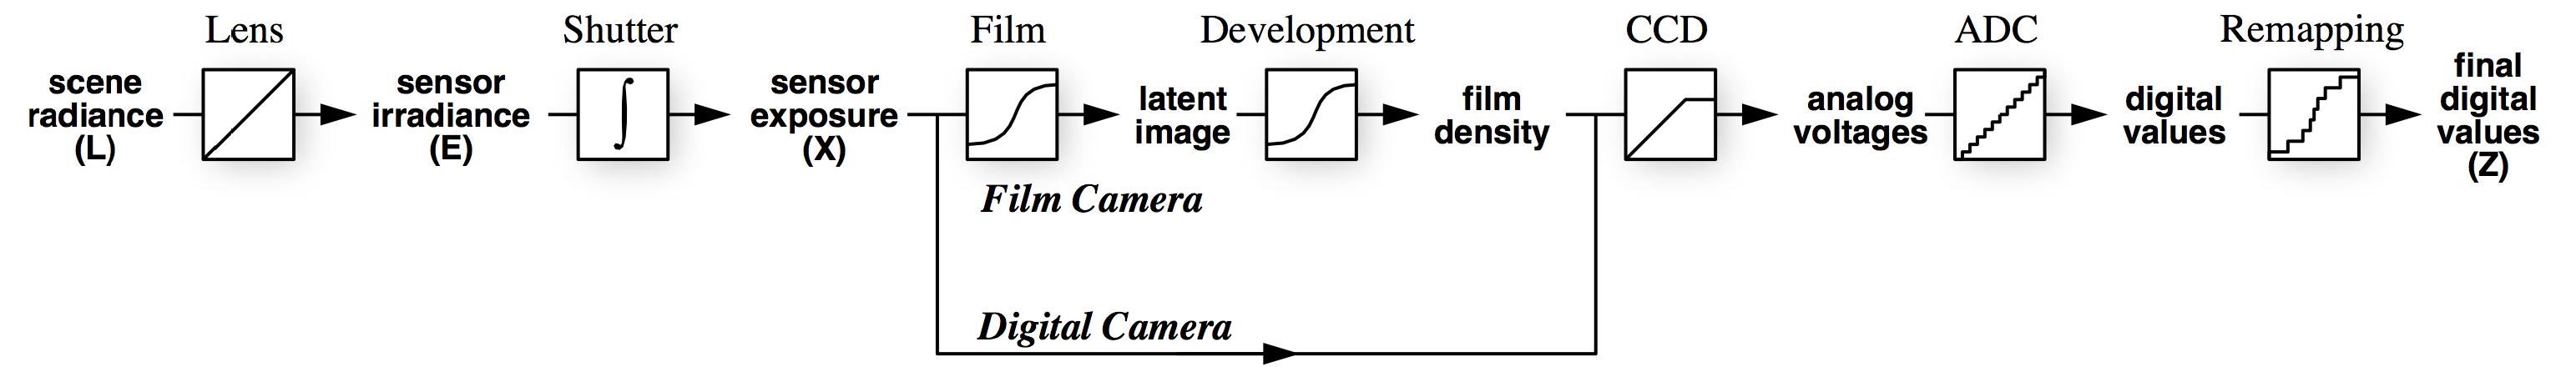
\includegraphics[width=\textwidth]{ImageAquisitionPipeline}
    \caption{Die Bildaufnahme Pipeline veranschaulicht, welche Prozesse durchlaufen werden bis aus einer realen Szene das digitale Bild für die Verwendung erzeugt wird (links nach rechts) \cite[S.2]{paper}}
    \label{fig:antwortkurve}
  \end{center}
\end{figure}


Trotz der allgemeinen Formulierung hat das Verfahren von Debevec und Malik jedoch auch einige Schwachstellen. Zum einen werden weder im Daten- noch im Glattheitsterm robuste Bestrafungsfunktionen verwendet. Diese könnten den Ansatz deutlich robuster unter Fehlmessungen machen. Zum werden keine Beschränkungen gefordert, die die typischerweise gewünschte Monotonie der Antwortkuve explizit erzwingen würden. Monotone Kurven können deshalb nur bei einer hinreichend großen Gewichtung der Glattheit erzielt werden. Schließlich ist das Verfahren auch nicht sonderlich robust gegenüber Rauschen. Dies kann insbesondere bei sehr kurz belichteten Bildern Probleme bereiten. 

\section{Aufgabenstellung}
Ziel der Arbeit ist es zunächst, das Verfahren von Debevec und Malik \cite{paper} als Ausgangsverfahren zu implementieren. Dies soll in einer dafür sinnvollen und portierbaren Programmiersprache umgesetzt werden.

Diese \nameref{chap:impl} soll dann sukzessive um robuste Funktionen, \gls{Monotonie}-Beschränkungen (siehe \autoref{sec:monotonie}) und räumliche Glattheitsterme (siehe \autoref{sec:raeumlich}) erweitert werden.

\begin{figure}[H]
  \begin{center}
    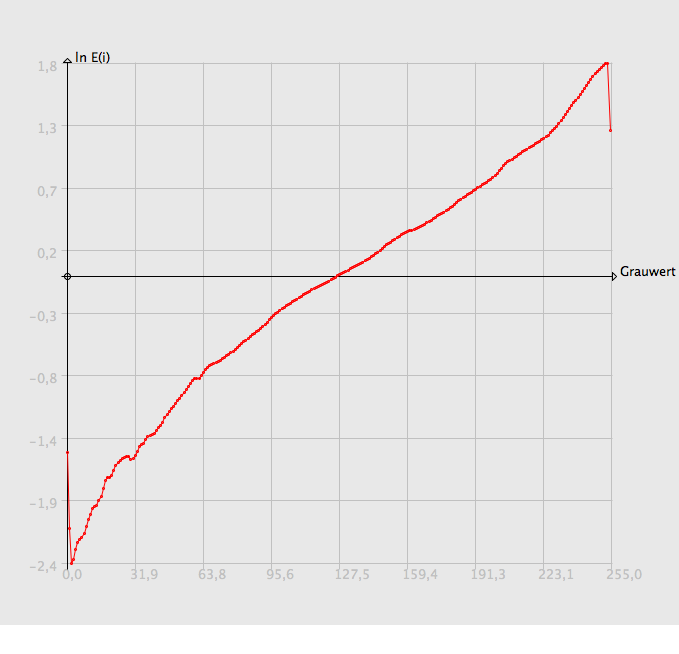
\includegraphics[width=0.45\textwidth]{teezer/g_noise_no_robustness}
    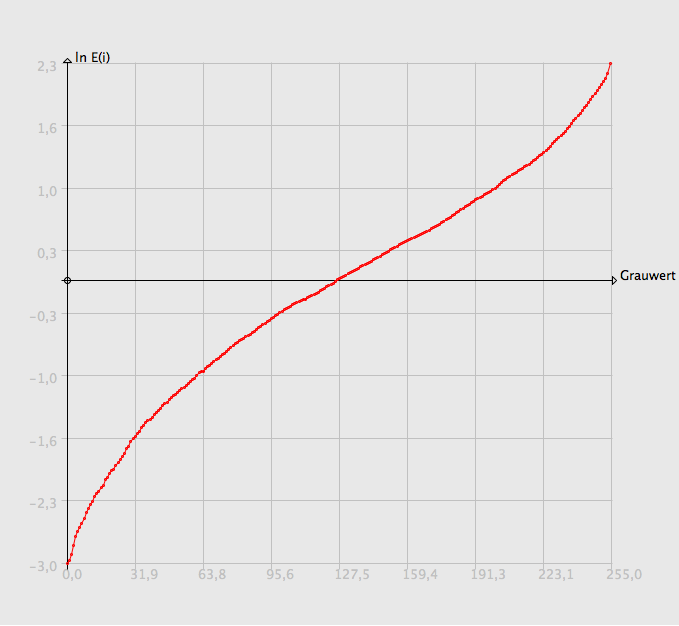
\includegraphics[width=0.45\textwidth]{teezer/g_noise_robustness_raum}
    \\
    \vspace{3pt}
    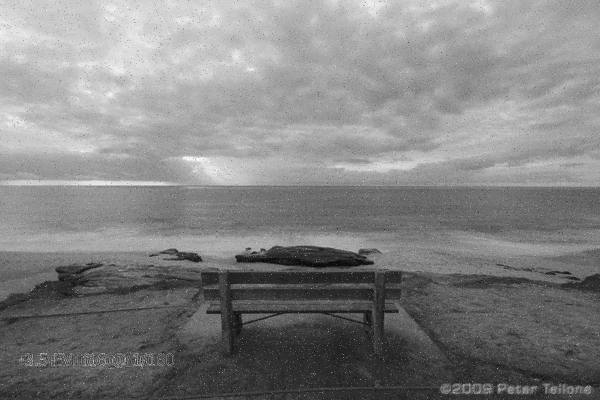
\includegraphics[width=0.45\textwidth]{teezer/E_noise_no_robustness}
    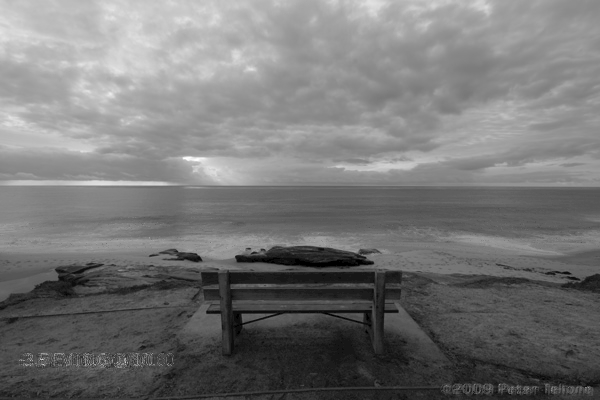
\includegraphics[width=0.45\textwidth]{teezer/E_noise_robustness_raum}
    \caption{Geschätzte Antwortkurven und zugehöriges HDR-Bild für die Bilderserie \cite{tellone} mit \gls{SaltAndPepperNoise}. \textbf{o.l.}: ohne robuste Bestrafungsterme. \textbf{o.r.}: mit robusten Bestrafungstermen und räumlicher Glattheitsforderung. \textbf{unten}: Das HDR-Bild wurde mittels lokalem Reinhard-Tone-Mapper (vgl. \autoref{sec:tone-mapping}) erstellt.}
    \label{fig:teezer}
  \end{center}
\end{figure}


Neben der Modellierung und Implementierung der einzelnen Erweiterungen soll auch eine geeignete visuelle Evaluation der Ergebnisse erfolgen. Hierzu sollen \gls{Tone-Mapping}-Verfahren (siehe \autoref{sec:tone-mapping}) aus bereits existierender Forschung verwendet werden. 


\section{Gliederung}
Die Arbeit ist in folgender Weise gegliedert:
\begin{description}

\item[\autoref{chap:hdr} -- \nameref{chap:hdr}:] Hier werden die Grundlagen der \gls{HDR}-Bilder vermittelt. Dabei wird auf die physikalischen, historischen und anwendungsorientierten Eigenschaften von \gls{HDR}-Bildern eingegangen.

\item[\autoref{chap:references} -- \nameref{chap:references}:] Anschließend werden verwandte Arbeiten zum Thema \gls{HDR} vorgestellt.

\item[\autoref{chap:algo} -- \nameref{chap:algo}:] Die zu Grunde liegende Vorgehensweise von Debevec und Malik \cite{paper} soll in diesem Kapitel beschrieben werden. Außerdem werden die existierenden Schwachstellen des bisherigen Ansatzes dargestellt.

\item[\autoref{chap:maths} -- \nameref{chap:maths}:] Der theoretische Ansatz aus \autoref{chap:maths} wird hier mathematisch umgesetzt und diskutiert. Außerdem werden die Erweiterungen des Algorithmus beschrieben und formal spezifiziert.

\item[\autoref{chap:impl} -- \nameref{chap:impl}:] Die Implementierung der in Kapitel \autoref{chap:algo} und \autoref{chap:maths} beschriebenen Modelle wird hier erläutert. Darüber hinaus werden einzelne Programm-Passagen (siehe \autoref{sec:sample-codes}) genauer beleuchtet und die Laufzeit der Anwendung (siehe \autoref{sec:laufzeit}) analysiert.

\item[\autoref{chap:results} -- \nameref{chap:results}:] Anschließend werden die Resultate und Einflüsse der unterschiedlichen Erweiterungen vorgestellt und diskutiert.

\item[\autoref{chap:zusfas} -- \nameref{chap:zusfas}:] Zusammenfassung der Ergebnisse der Arbeit und Darstellung von Anknüpfungspunkte zu weiteren Arbeiten.
\end{description}
